\section{Conclusion}
We have examined different designs of Tangible User Interfaces in this report. Furthermore, we have presented and discussed several examples of TUIs. Although the focus of this work lies in TUIs for visualization, we have also presented TUIs for other domains. A discussion about different aspects of TUIs followed their presentation. 

TUIs can be intuitive tools for the examination of visualized data. Instead of using the classic mouse and keyboard interaction, they enable users a more natural way of exploration and interaction with digital content. By using graspable objects and multi-touch gestures, users learn the interaction patterns more easily. This results in a faster and more comfortable way of examining visualized information. The TUI interaction paradigms work especially well for huge amount of data with multiple layers. However, TUIs are normally specialized on certain visualization tasks. Therefore, TUIs can only interact with certain styles of visualizations effectively. Everyday tasks like writing or navigating through documents or searching the web are still accomplished faster with traditional ways of computer interaction.

%should be on top of last page
\begin{figure}
\centering
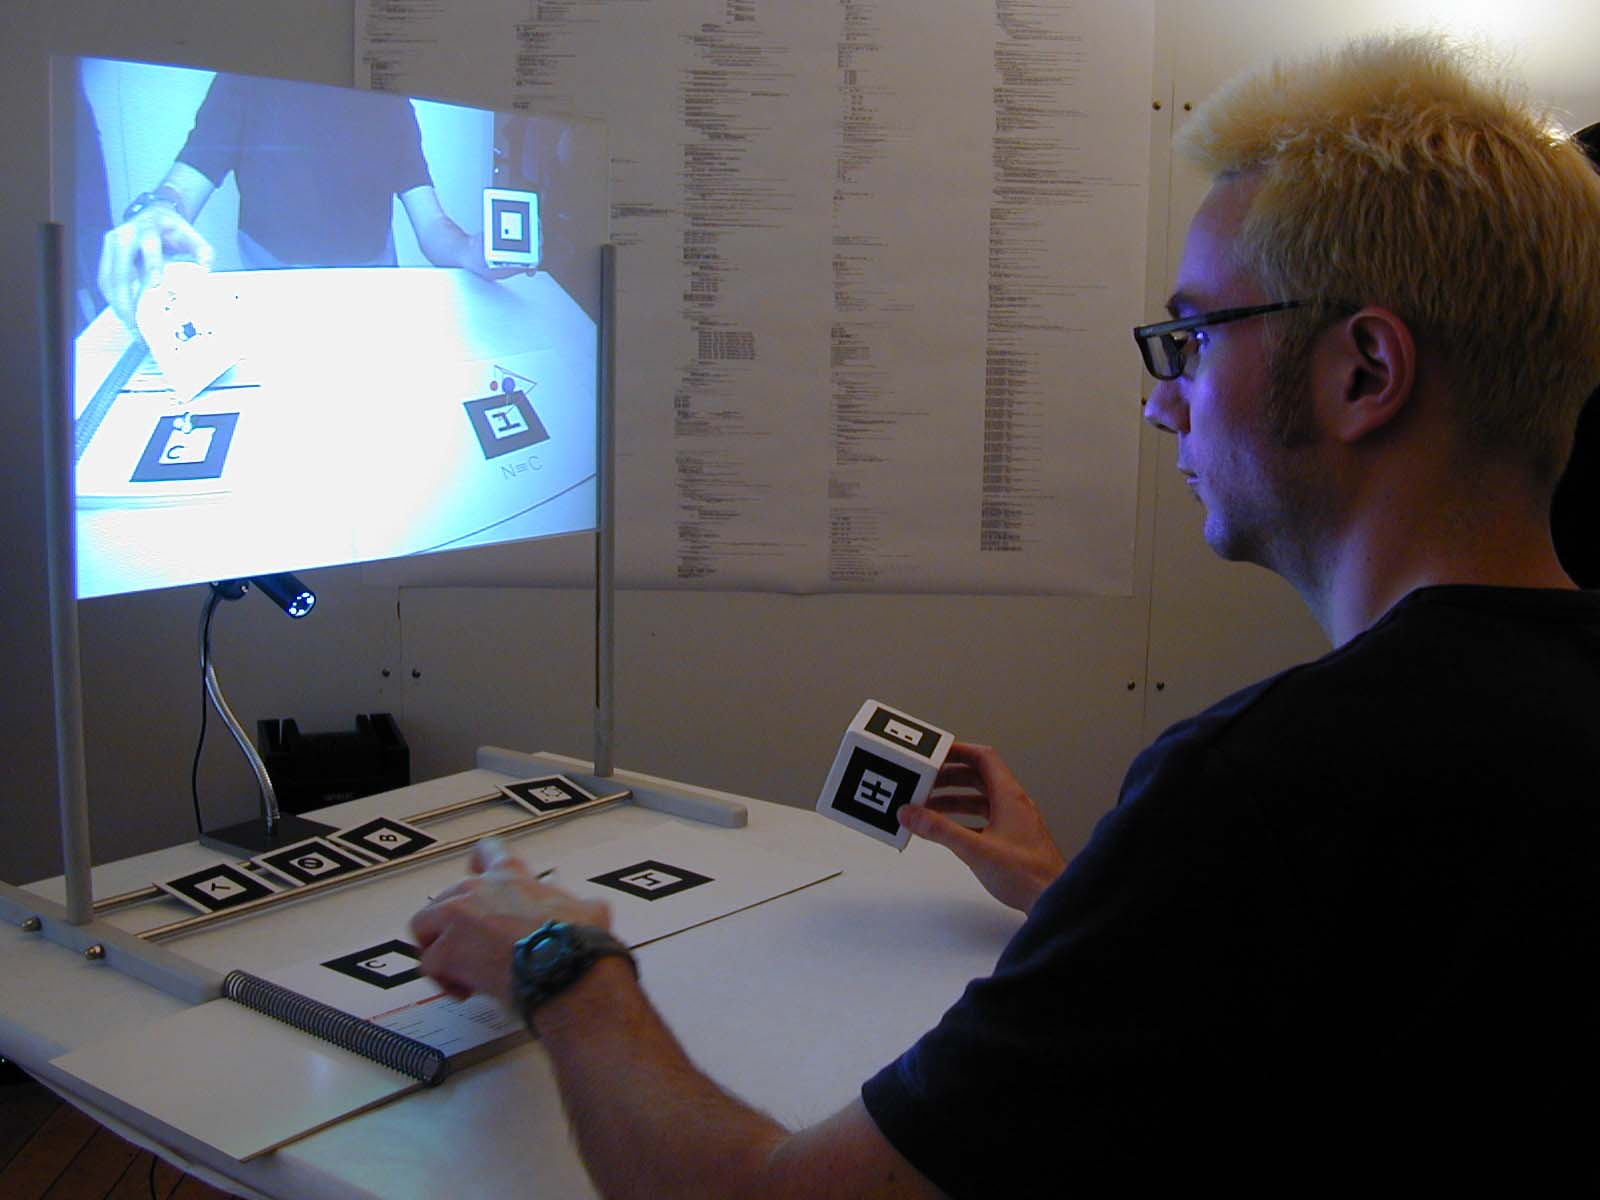
\includegraphics[width=0.47\textwidth]{figures/augmented_chemistry.jpg}
\caption{Augmented Chemistry in action (compare \protect\cite{fjeld02})}
\label{fig:augmented_chemistry}
\end{figure}